\subsection{Подсистема Цены поставщиков}
\subsubsection{Описание подсистемы Цены поставщиков}
Согласно поставленной задаче необходимо хранить цены поставщиков по которым достигнута договоренность, для осуществления контроля правильности закупочных цен при поступлении товаров. Так же  необходимо предусмотреть действия в случае некорректных цен  в документах <<Поступление ТМЦ>>. 
\par
Так как в следующих задачах пойдет речь о ценах конкурентов  (см.\hyperlink{5_1}{\textit {"Подсистема Цены конкурентов"}}), то мы обобщим и будем говорить не о ценах ,,поставщиков`` или ,,конкурентов``, а о ценах ,,Контрагентов``.  
\par
В документ ,,Поступления ТМЦ`` в табличную часть ,,Товары`` будут добавлены две дополнительные колонки:
\begin{itemize}	
	\item ,,ЦенаДоговорная``
	\item ,,РасхождениеЦен``
\end{itemize}		
Колонка ,,ЦенаДоговорная`` будет заполнена ценами номенклатуры установленные как ,,ДоговорныеЗакупочные``, а колонка ,,РасхождениеЦен`` разницей в цене между ценой указанной в приходном документе и ценой по которой поставщик согласно договора должен нам отпустить товар.	Такой подход позволит оперативно, ещ в непроведенном документе поступления увидеть есть ли ошибки в отпускных ценах. На основании этой информации могут быть приняты управленческие решения.
\subsubsection{Реализация подсистемы Цены поставщиков}
\paragraph{Добавления в системе:}
\begin{itemize}	
	\item \label{l1}Периодический регистр сведений ,,Цены номенклатуры контрагентов``, хранящий цены в разрезе контрагента, типа его цены  и магазина.
	\begin{figure}[H]
		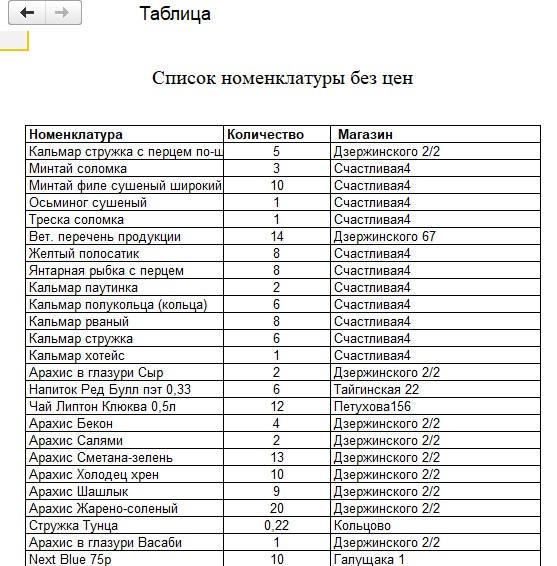
\includegraphics[width=0.3\textwidth]{3.jpg}
		\caption{Структура регистра.}
		\label{ris:3.jpg}
	\end{figure}
	\begin{figure}[H]
		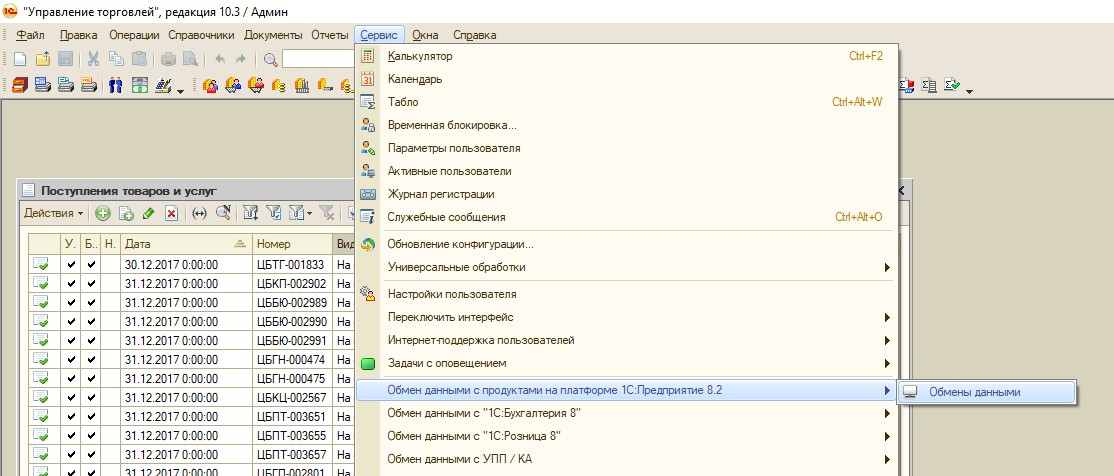
\includegraphics[width=0.6\textwidth]{1.jpg}
		\caption{Цены номенклатуры контрагентов.}
		\label{ris:1.jpg}
	\end{figure}
	\begin{figure}[H]
		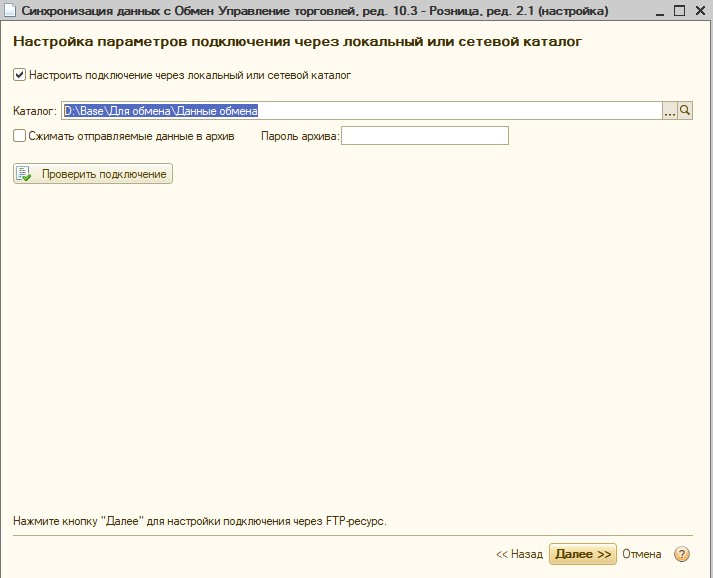
\includegraphics[width=0.8\textwidth]{6.jpg}
		\caption{Структура данных регистра.}
		\label{ris:6.jpg}
	\end{figure}
	\item Справочник ,,ТипыЦенНоменклатурыКонтрагентов``. Справочник подчинен справочнику ,,Контрагенты``. и хранит типы цен номенклатуры в разрезе контрагентов, наименований, типов цены  и магазина. 
	\begin{figure}[H]
		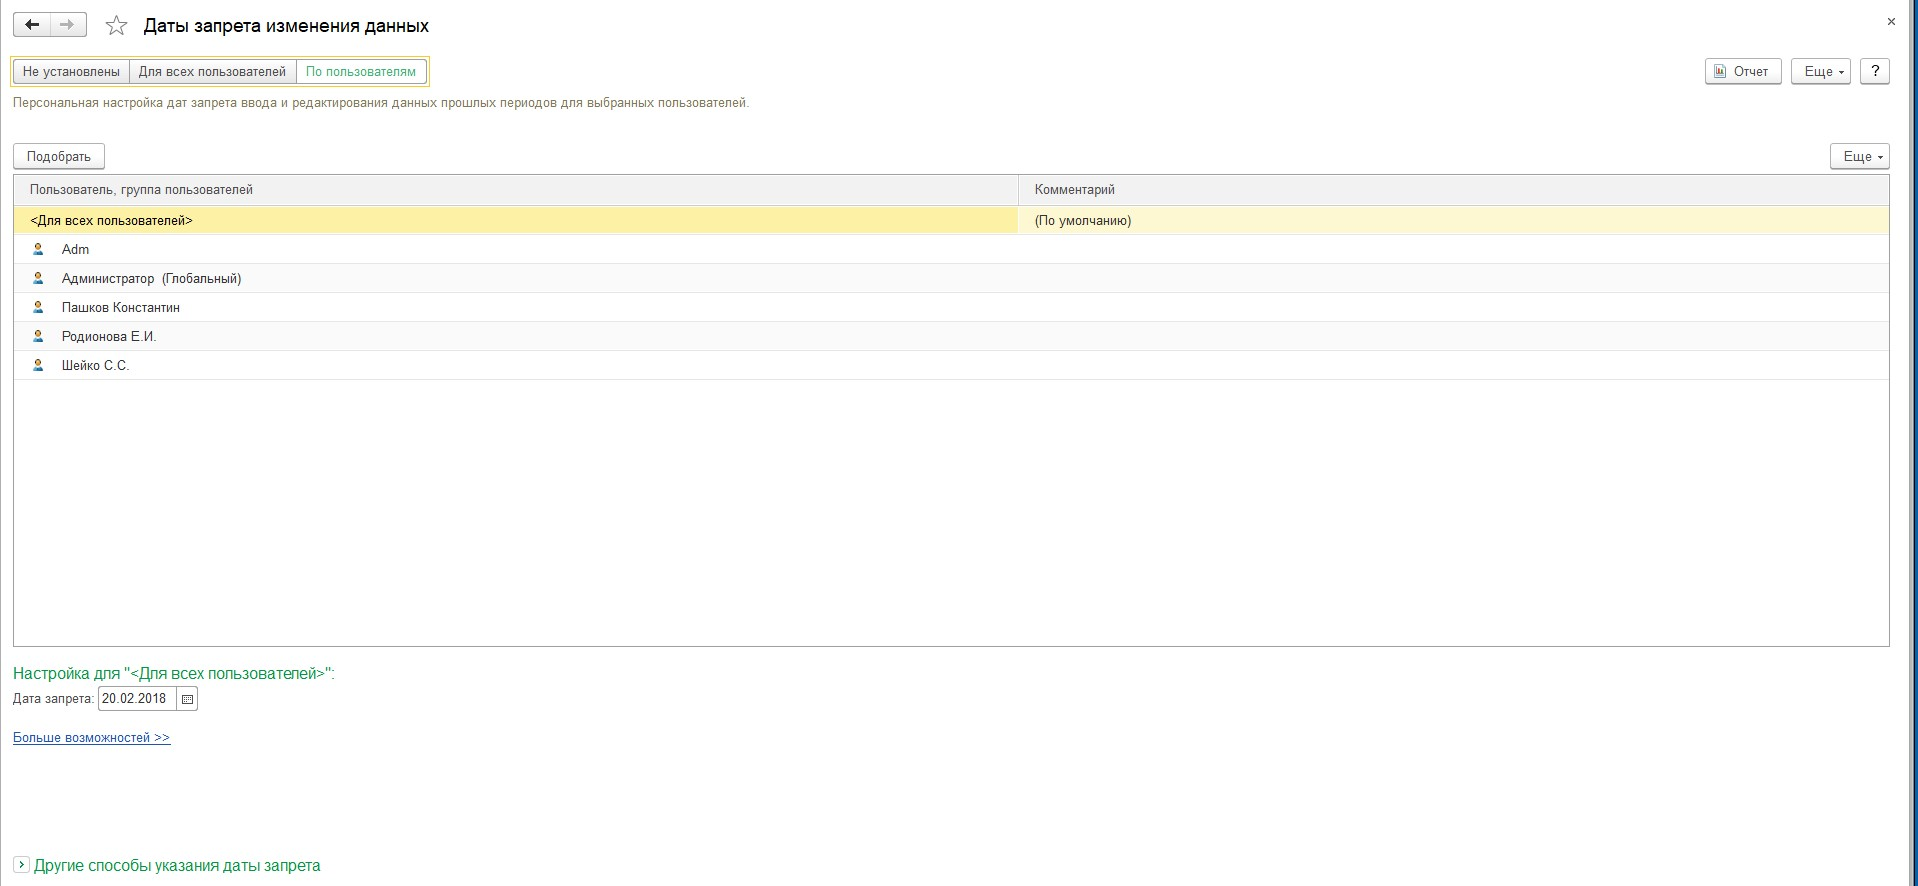
\includegraphics[width=0.4\textwidth]{4.jpg}
		\caption{Структура справочника.}
		\label{ris:4.jpg}
	\end{figure}
	\begin{figure}[H]
		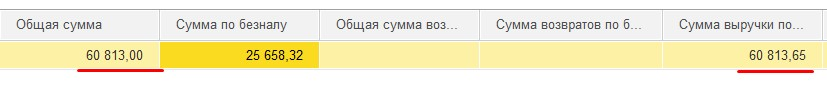
\includegraphics[width=0.8\textwidth]{5.jpg}
		\caption{Cправочник.}
		\label{ris:5.jpg}
	\end{figure}

	\begin{figure}[H]
		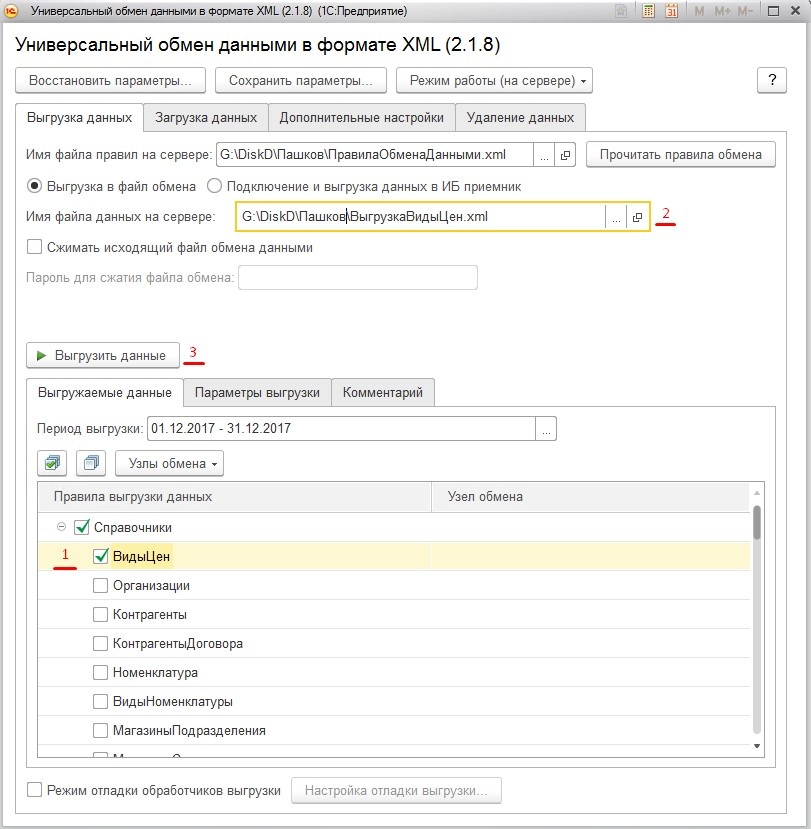
\includegraphics[width=0.8\textwidth]{7.jpg}
		\caption{Cправочник структура данных.}
		\label{ris:7.jpg}
	\end{figure}
	\item Документ ,,Установка цен номенклатуры контрагентов`` (Документ позволяет зафиксировать цену контрагента на позицию номенклатуры на определенную дату). Документ создается на основе типового документа ,,Установка цен номенклатуры``. В него добавляется новый реквизит -- <<Контрагент>> 
	   (Рис.~\ref{ris:2.jpg}), документ формирует движения по регистру \hyperref[l1]{,,ЦеныНоменклатурыКонтрагентов``}. 
	
	\begin{figure}[H]
		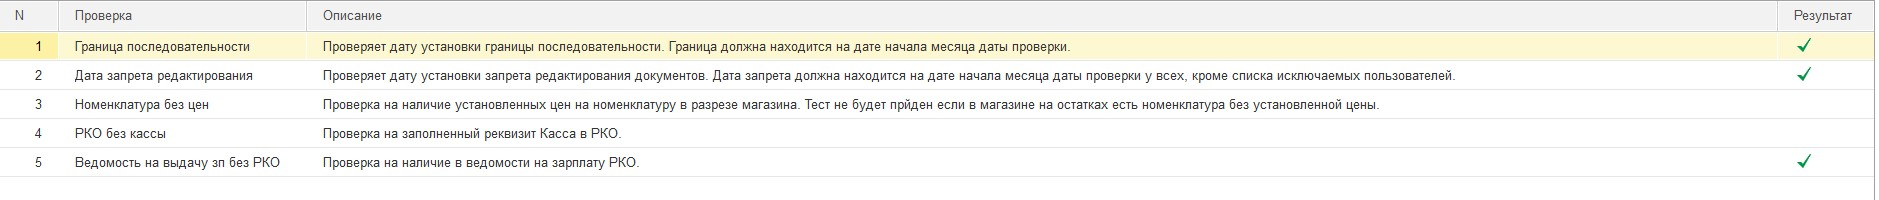
\includegraphics[width=0.6\textwidth]{2.jpg}
		\caption{Установка цен номенклатуры контрагентов.}
		\label{ris:2.jpg}
	\end{figure}
	
\end{itemize}
\paragraph{Изменения в системе:}
\begin{enumerate}	
	\item В документ ,,Поступления ТМЦ`` в табличную часть ,,Товары`` добавить колонки ,,ЦенаДоговорная`` и ,,РасхождениеЦен``. Заполнять или изменять ее при изменении номенклатуры, если на номенклатуру отсутствует договорная цена поставщика устанавливать значение в соответствующей строке в <<0>>.
	В колонке ,,РасхождениеЦен`` фиксируется разница между ценой закупки и ценой поставщика.
	
	\item При записи документа проводить проверку на то, что цена указанная в приходном документе отличается от установленной на дату документа цены поставщика.
	\item Принятие мер для устранение проблемы. Возможные меры: 
	\begin{itemize}	
			\item \textit{Выдается дополнительное сообщение пользователю, документ проводится, но на электронную почту ответственного лица отправляется сообщение о расхождении цен. Возникает вопрос, если документ все-таки проводить, откуда брать цены для расчета себестоимости. Брать ошибочную цену из документа нельзя, брать цену поставщика, нужно переписывать модуль проведения в части расчета себестоимости.}
		\begin{figure}[H]
			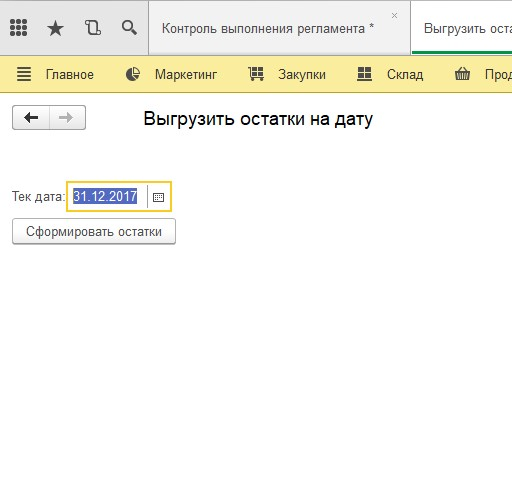
\includegraphics[width=0.6\textwidth]{9.jpg}
			\caption{Вариант 1.}
			\label{ris:9.jpg}
		\end{figure}		
			\item \textit{Выдается дополнительное сообщение пользователю, проведение документа блокируется, до изменения цены закупки. На электронную почту ответственного лица отправляется сообщение о расхождении цен. }
		\begin{figure}[H]
			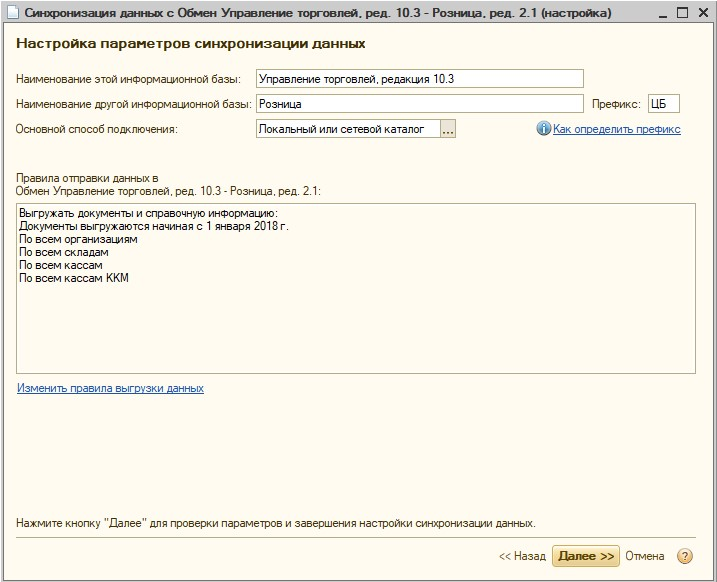
\includegraphics[width=0.6\textwidth]{8.jpg}
			\caption{Вариант 2.}
			\label{ris:8.jpg}
		\end{figure}		
		\item \textit{Рассмотреть еще возможные варианты.}
	\end{itemize}
\end{enumerate}
\paragraph{Вопросы:}
\begin{itemize}	
	\item \emph{Если товар пришел со скидкой, т.е. цена поставщика выше закупочной. Действия в этом случае? (как это повлияет на себестоимость в плане того из какой колонки документа брать цены? )}
	\item \emph{Если на момент формирования документа ,,Поступления ТМЦ`` цены поставщика отсутствуют, действия в этом случае?}
	\item \emph{Какое ответственное лицо и на основании каких документов будет заполнять документ ,,Установка цен номенклатуры контрагентов``?} \par \emph{Что будет являться основанием для изменения цен поставщика?}
\end{itemize}
%\begin{itemize}
%	\item Необходимо хранение договорных цен поставщиков на отдельную номенклатуру, контроль договорных цен в п 
	
	
	
%\end{itemize}	

%\subsubsection{Реализация подсистемы "Цены поставщиков"}

%\begin{enumerate}	
%	\item Обработка восстановления последовательности находится в меню, в разделе "Все функции" %Рис.~\ref{ris:1.jpg}
%	\begin{figure}[H]
%		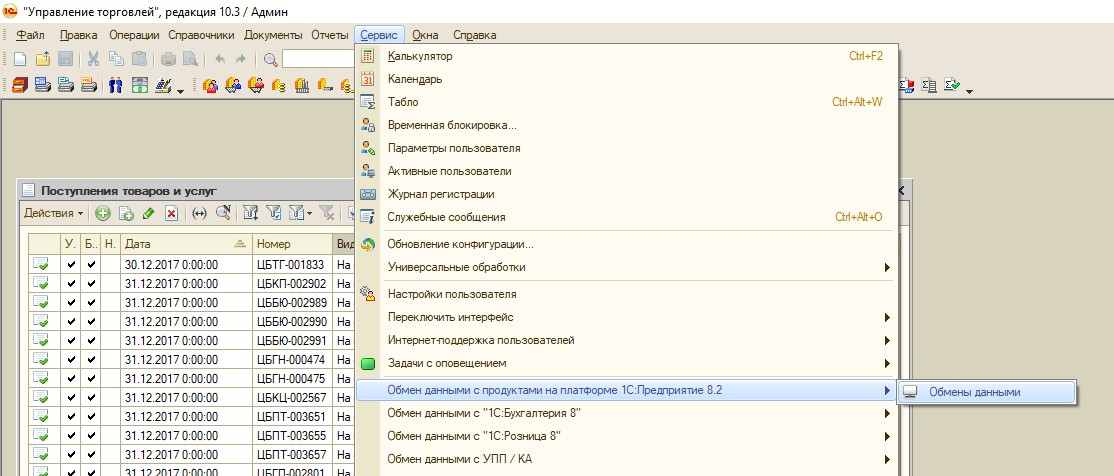
\includegraphics[width=0.19\textwidth]{1.jpg}
%		\caption{Расположение меню "Всё функции".}
%		\label{ris:1.jpg}
%	\end{figure}
%	В этой форме нас интересует пункт "Стандартные" Рис.~\ref{ris:2.jpg}

%	\item Внимание! Восстановление последовательности может занять длительное время.
%\end{enumerate}

